\documentclass[10pt, conference]{IEEEtran}
\usepackage[english]{babel}
\usepackage[usenames]{color}
\usepackage{colortbl}
\usepackage{comment}
\usepackage{graphicx}
\graphicspath{ {figures/} }
\usepackage{epsfig}
\usepackage{array, colortbl}
\usepackage{listings}
\usepackage{epstopdf}
\usepackage{multirow}
\usepackage{rotating}
%\usepackage{subfigure}
\usepackage{subfig}
\usepackage{float}
\usepackage[obeyspaces,hyphens,spaces]{url}
\usepackage{balance}
\usepackage{fancybox}
\usepackage{scalefnt}
\usepackage[normalem]{ulem}
%\pagestyle{plain}
\pagenumbering{arabic}
\pagestyle{empty}
\clubpenalty = 10000
\widowpenalty = 10000
\displaywidowpenalty = 10000
\usepackage{cleveref}

\newtheorem{hypothesis}{Hypothesis}
\newtheorem{nullhypothesis}{Null Hypothesis}


\makeatletter
\renewcommand{\paragraph}[1]{\noindent\textsf{#1}.}

\title{Assignement 1}
\author{Billy Bouchard$^{1}$
    \\
    \emph{$^{1}$  M.S. computer engineering, Polytechnique Montreal}}

\begin{document}
\maketitle


\section{Introduction}
\label{sec:introduction}

CPU times are one of the most monitored statistics of all in computer science.
It gives a lot of information about how the system resources are distributed, what tends to be a performance bottleneck and what kind of requests are the most done by clients. 
Therefore, having a robust way of analysing cpu data is important to better understand a system.
This report will focus on some basic analysis techniques of 2 different CPU time datasets.
It will try to answer 4 questions : 
\begin{enumerate}
    \item Are the performance data (i.e., CPU usage) normally distributed?
    \item Does there exist statistically significance difference between the performance of the two versions?
    \item How large is the difference if it exits?
    \item Does the performance change over time?
\end{enumerate}

\section{Approach}
\label{sec:approach}

A simple analytical study using Python would be enough to answer all the questions.
Therefore, the first question would be answered by doing two histograms of the TOTAL\_CPU column.
To answer the second question, we will need to see whether they are normally distributed or not. 
If they are, one can use a dependent (paired) two-sample t-test.
If not, a Wilcoxon signed-rank test would be used.
To answer the third question, cohen's D test can be used for normal distribution otherwise the cliff's delta would be best.
Finally, the fourth question can be answered with the Mann-Kendall trend test for each different set of data.

Of all those questions we shall emit 2 null hypotheses first one of which will be that 
\begin{nullhypothesis}
    There exists no relation/correlation between the original and the new data.
\end{nullhypothesis} 
Since both are data that come from a server, it makes sense that a certain correlation exists between them.
The second one. 
\begin{nullhypothesis}
    Over time, the average time to answer a request will be augmented.
\end{nullhypothesis} 
 If a system is well-optimized, there shouldn't be any issues with a large amount of requests. Therefore, the time should stay pretty consistent.

\section{Results}
\label{sec:results}

\begin{figure}[h]
    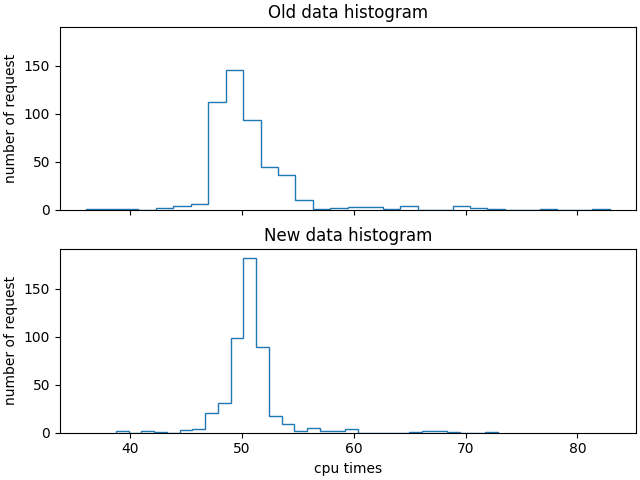
\includegraphics[width=8cm]{histograms.png}
    \caption{Histograms of new and original data}
    \label{fig:hist}
\end{figure}

The first question was answered by doing a simple histogram of both data that can be seen in figure \ref{fig:hist}. 
Distributions seem normal at first glance, but there are strong outliers on the right side of the curve which makes it derive from a normal distribution. 
However, since this study does not discriminate the data, we shall not remove any outliers and consider the data as a whole.

Since the data distribution resembled a normal distribution, both the t-test and the Wilcoxon test have been made with the data. 
Results can be found in table \ref{tab:res23}.
This proves the fact that they do not seem to follow a normal distribution as the Wilcoxon test has a very small p-value compared to the T-test.
However, from the data, it is clear that there is a correlation between both data.
Thus, we can reject our null hypothesis 1, showing that there is a correlation.

To answer the third question, we also did both Cohen's D and Cliff's delta and the results can be seen in table \ref{tab:res23}. 
However, based on the prior observations, it is probable that only Cliff's delta is accurate. 
The numbers show that there is only a small difference between both data sets.

Finally, to answer the fourth question,  Mann Kendall test was executed on each data set to see what trend each one had.
As was thought, no trend was observed even though the p-value for the original data came dangerously low.
Therefore, we can reject our second null hypothesis and state that there is no trend in both data sets.

\begin{table}
    \centering
    \begin{tabular}[h]{|l|l|}
        \hline
        \textbf{Test done} &  \textbf{value} \\ \hline \hline
        Wilcoxon & 0.0025  \\ \hline 
        T-test & 0.5942 \\ \hline \hline
        cohen's D & -0.0352 \\ \hline 
        cliff's delta & -0.1976 \\ \hline 
    \end{tabular}        
    \caption{Results of the different test done on comparing both data}
    \label{tab:res23}
\end{table}

\begin{table}
    \centering
    \begin{tabular}[h]{|l|l|l|}
        \hline
        \textbf{Test done} &  \textbf{original data} & \textbf{new data} \\ \hline
        Mann Kendalls test & 0.0596 & 0.2875 \\ \hline 
    \end{tabular}        
    \caption{Trend analysis of both data set}
    \label{tab:trend}
\end{table}

\section{Replication}
\label{sec:replication}

All of this study, including the code and data can be replicated. 
These can be found at \verb|https://github.com/34yu34/log6309e-assignement1|.
Running the analysis.py program will show all the calculation done.

\section{Conclusion}
\label{sec:conclusion}

In conclusion, We were able to reject our first null hypothesis proving that there is a correlation between the original data and the new data. 
Moreover, the trend test confirms that there is no trend inside the data which lets us reject the second null hypothesis.
However, small outliers in the data might have affected some of the tests.
It would be interesting to redo the analysis of the data set once a couple of data analysis techniques have been executed on it. 


\balance
%\bibliographystyle{IEEEtran}
%\bibliography{assignment.bib}
\end{document}
